%% ==============================================================
%% DIRECT ACYCLIC GRAPH
%% ==============================================================

\begin{figure}[t]
\centering
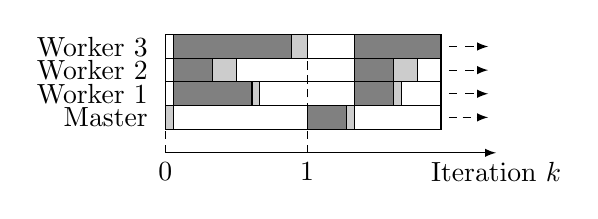
\begin{tikzpicture}
% Worker 1
\draw[black] (0,0.4) rectangle (0.1,0.7);
\draw[black,fill=gray!100](0.1,0.4) rectangle (1.1,0.7); % cd = 0.5, td = 0.1
\draw[black,fill=gray!40] (1.1,0.4) rectangle (1.2,0.7);
\draw[black] (1.2,0.4) rectangle (2.4,0.7);
\draw[black,fill=gray!100](2.4,0.4) rectangle (2.9,0.7);
\draw[black,fill=gray!40](2.9,0.4) rectangle (3,0.7);
\draw[black] (3,0.4) rectangle (3.5,0.7);
\draw[dashed,->,>=latex] (3.6,0.55) -- (4.1,0.55); 

% Worker 2
\draw[black](0,0.7) rectangle (0.1,1);
\draw[black,fill=gray!100](0.1,0.7) rectangle (0.6,1); % cd = 0.5, td = 0.3
\draw[black,fill=gray!40] (0.6,0.7) rectangle (0.9,1);
\draw[black](0.9,0.7) rectangle (2.4,1);
\draw[black,fill=gray!100](2.4,0.7) rectangle (2.9,1);
\draw[black,fill=gray!40] (2.9,0.7) rectangle (3.2,1);
\draw[black](3.2,0.7) rectangle (3.5,1);
\draw[dashed,->,>=latex] (3.6,0.85) -- (4.1,0.85); 

% Worker 3
\draw[black](0,1) rectangle (0.1,1.3);
\draw[black,fill=gray!100](0.1,1) rectangle (1.6,1.3); % cd = 1.5, td = 0.2
\draw[black,fill=gray!40] (1.6,1) rectangle (1.8,1.3);
\draw[black] (1.8,1) rectangle (2.4,1.3);
\draw[black,fill=gray!100](2.4,1) rectangle (3.5,1.3);
\draw[dashed,->,>=latex] (3.6,1.15) -- (4.1,1.15); 

% Master
\draw[black,fill=gray!40] (0,0.1) rectangle (0.1,0.4); % cd = 0.5, td = 0.1
\draw[black] (0.1,0.1) rectangle (1.8,0.4);
\draw[black,fill=gray!100] (1.8,0.1) rectangle (2.3,0.4);
\draw[black,fill=gray!40] (2.3,0.1) rectangle (2.4,0.4);
\draw[black](2.4,0.1) rectangle (3.5,0.4);
\draw[densely dashed,->,>=latex] (3.6,0.25) -- (4.1,0.25); 

% Axis
\node[below] (k1)  at (1.8,-0.2) {$1$};
\draw[->,>=latex] (0,-0.2) -- (4.2,-0.2) node[below]{Iteration $k$} ;

% Vertical lines
\draw[densely dashed] (0,-0.2) -- (0,1.3);
\draw[densely dashed] (1.8,-0.2) -- (1.8,1.3);   

% Names
\node[below] (axis) at (0,-0.2) {$0$};
\node[left] (M)  at (-0.1,0.25) {Master};
\node[left] (W1) at (-0.1,0.55) {Worker 1};
\node[left] (W2) at (-0.1,0.85) {Worker 2};
\node[left] (W3) at (-0.1,1.15) {Worker 3};
\end{tikzpicture}
\caption{Illustration of a synchronous distributed mechanism (idle time in white, transmission delay in light gray, computation delay in gray). The master is triggered once it has received information from all the workers.}
\label{fig:sync}
\end{figure}
